\documentclass[tikz,border=6pt]{standalone}
\usepackage{tikz}
\usetikzlibrary{arrows.meta,positioning,calc}

%% fonts
\usepackage{dsfont}
\usepackage{newpxtext}
\usepackage{newpxmath}
\usepackage{amsmath}
\usepackage{caption}

% --- colors & styles ---
\definecolor{incolor}{RGB}{255,194,120}   % soft orange
\definecolor{hidcolor}{RGB}{173,173,255}  % soft violet
\definecolor{outcolor}{RGB}{255,180,180}  % soft red

% node radius & scatter used for straight-line end-pointing
\def\noderad{9mm} 
\def\scatter{1.0} % tiny degrees; adjust 0.6–1.2 for more/less separation

\tikzset{
  nnnode/.style = {circle, minimum size=14mm, inner sep=0pt, font=\Large},
  input/.style  = {nnnode, fill=incolor},
  hidden/.style = {nnnode, fill=hidcolor},
  output/.style = {nnnode, fill=outcolor},
  dots/.style   = {nnnode, fill=white, draw=none, font=\Large},
  conn/.style   = {-{Stealth[length=2.5mm,width=2.0mm]},
                   line width=1pt, draw=gray!70,
                   shorten >=-0.5mm, shorten <=-0.5mm},
  collabel/.style = {font=\Large, align=center}
}

\begin{document}
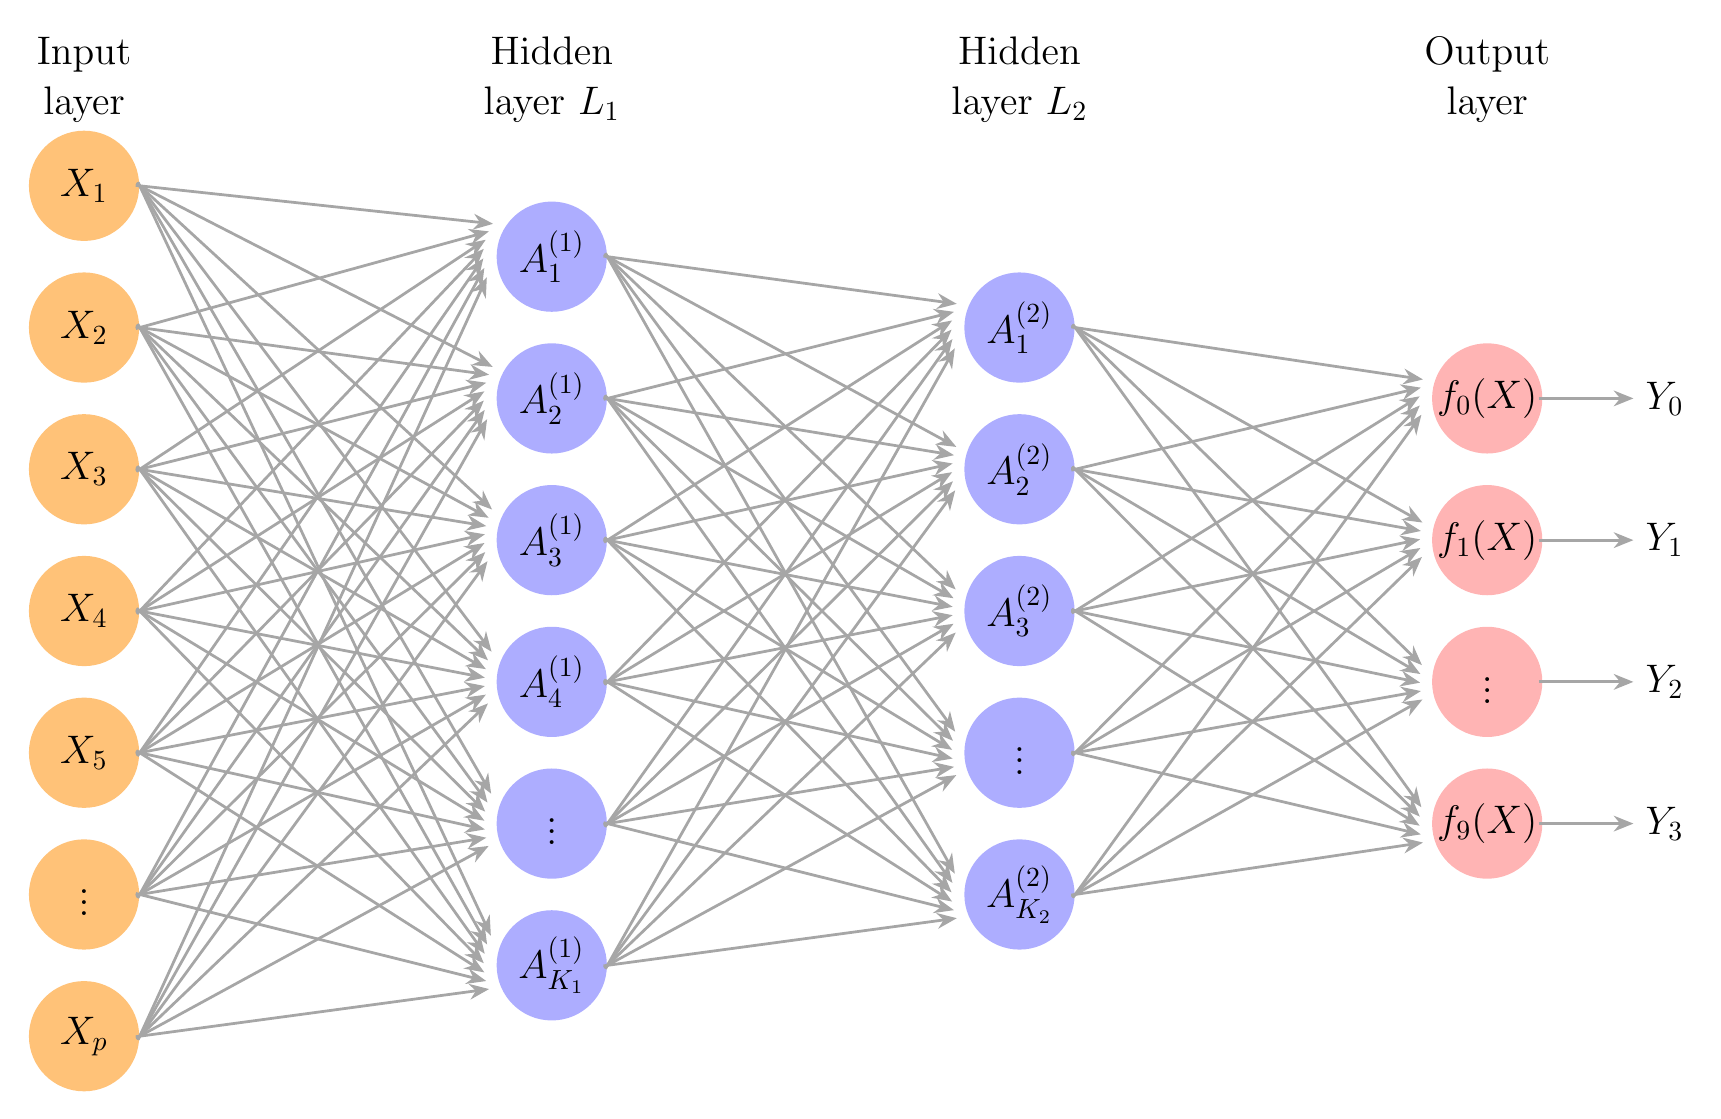
\begin{tikzpicture}[x=2.2cm,y=0.9cm]

% column titles
\node[collabel] at (0,  7.5) {Input\\ layer};
\node[collabel] at (2.7,7.5) {Hidden\\ layer $L_1$};
\node[collabel] at (5.4,7.5) {Hidden\\ layer $L_2$};
\node[collabel] at (8.1,7.5) {Output\\ layer};

% -------------------- Nodes --------------------

% Input layer: X1, X2, X3, X4, X5, dots, Xp
\foreach \y/\name [count=\mi] in {6/{$X_{1}$}, 4/{$X_{2}$}, 2/{$X_{3}$}, 0/{$X_{4}$},
                                  -2/{$X_{5}$}, -4/{$\vdots$}, -6/{$X_{p}$}}{
  \node[input] (x\mi) at (0,\y) {\name};
}

% Hidden layer L1: A^{(1)}_1 ... A^{(1)}_{K1} with dots
\foreach \y/\name [count=\mj] in {5/{$A^{(1)}_{1}$}, 3/{$A^{(1)}_{2}$}, 1/{$A^{(1)}_{3}$},
                                  -1/{$A^{(1)}_{4}$}, -3/{$\vdots$}, -5/{$A^{(1)}_{K_{1}}$}}{
  \node[hidden] (hOne\mj) at (2.7,\y) {\name};
}

% Hidden layer L2: A^{(2)}_1 ... A^{(2)}_{K2} with dots
\foreach \y/\name [count=\mk] in {4/{$A^{(2)}_{1}$}, 2/{$A^{(2)}_{2}$}, 0/{$A^{(2)}_{3}$},
                                  -2/{$\vdots$}, -4/{$A^{(2)}_{K_{2}}$}}{
  \node[hidden] (hTwo\mk) at (5.4,\y) {\name};
}

% Output layer: f_0(X), f_1(X), dots, f_9(X)
\foreach \y/\name [count=\mo] in {3/{$f_{0}(X)$}, 1/{$f_{1}(X)$}, -1/{$\vdots$}, -3/{$f_{9}(X)$}}{
  \node[output] (out\mo) at (8.1,\y) {\name};
  % right-hand arrow to Y_i label
  \draw[conn] (out\mo.east) -- ++(0.5,0)
    node[right=2pt,font=\Large] {$Y_{\the\numexpr\mo-1\relax}$};
}

% -------------------- Connections (straight with tiny angular scatter) --------------------

% Input -> Hidden L1
\foreach \mi in {1,...,7}{                 % 8 input nodes (incl. \vdots)
  \foreach \mj [count=\n] in {1,2,3,4,5,6}{% 5 L1 nodes (incl. \vdots)
    \pgfmathsetmacro{\ang}{180 + (\mi-4.5)*\scatter*8} % small spread
    \draw[conn] (x\mi.east) -- ($(hOne\n)+(\ang:\noderad)$);
  }
}

% Hidden L1 -> Hidden L2
\foreach \mj in {1,...,6}{
  \foreach \mk [count=\n] in {1,2,3,4,5}{
    \pgfmathsetmacro{\ang}{180 + (\mj-3.5)*\scatter*8}
    \draw[conn] (hOne\mj.east) -- ($(hTwo\n)+(\ang:\noderad)$);
  }
}

% Hidden L2 -> Output
\foreach \mk in {1,...,5}{
  \foreach \mo [count=\n] in {1,2,3,4}{
    \pgfmathsetmacro{\ang}{180 + (\mk-3)*\scatter*8}
    \draw[conn] (hTwo\mk.east) -- ($(out\n)+(\ang:\noderad)$);
  }
}

\end{tikzpicture}
\end{document}
